
%(BEGIN_QUESTION)
% Copyright 2004, Tony R. Kuphaldt, released under the Creative Commons Attribution License (v 1.0)
% This means you may do almost anything with this work of mine, so long as you give me proper credit

Calculate all voltages, currents, and total power in this balanced Y-Delta system:

$$\includegraphics[width=15.5cm]{i02299x01.eps}$$

\begin{itemize}
\item{} $E_{line} =$
\vskip 10pt
\item{} $I_{line} =$
\vskip 10pt
\item{} $E_{phase(source)} =$
\vskip 10pt
\item{} $I_{phase(source)} =$
\vskip 10pt
\item{} $E_{phase(load)} =$
\vskip 10pt
\item{} $I_{phase(load)} =$
\vskip 10pt
\item{} $P_{total} =$
\end{itemize}

\vskip 20pt \vbox{\hrule \hbox{\strut \vrule{} {\bf Suggestions for Socratic discussion} \vrule} \hrule}

\begin{itemize}
\item{} Explain how you may double-check your quantitative answer(s) with a high degree of confidence (i.e. something more rigorous than simply re-working the problem again in the same way).
\end{itemize}

\underbar{file i02299}
%(END_QUESTION)





%(BEGIN_ANSWER)

\begin{itemize}
\item{} $E_{line} =$ 207.8 V
\item{} $I_{line} =$ 0.621 A
\item{} $E_{phase(source)} =$ 120 V
\item{} $I_{phase(source)} =$ 0.621 A
\item{} $E_{phase(load)} =$ 207.8 V
\item{} $I_{phase(load)} =$ 0.358 A
\item{} $P_{total} =$ 223.4 W
\end{itemize}

%(END_ANSWER)





%(BEGIN_NOTES)

Be sure to ask your students to describe {\it how} they arrived at the answers to this question.  There is more than one place to start in determining the solution here, and more than one way to calculate some of the figures.  No matter how your students may have approached this question, though, they should all obtain the same answers.

%INDEX% Electronics review: 3-phase voltage/current/power calculation

%(END_NOTES)



